\section{Update}\label{model-update}
Before we discuss sampling, we will first discuss how to update a model.
We will assume that our detection step in the previous section has selected 
a set of candidate records $R_{dirty}$ and our sampling step has sampled from this
set of candidate records.
We will show that this model update procedure can be interpreted as a Stochastic 
Gradient Descent (SGD) algorithm, which gives us a theoretical framework to analyze
convergence and bound the error at each step.

\subsection{Update Problem}
The challenge is that we want a model update technique that takes advantage of the entire dirty data and a small sample of cleaned data.
However, we want to avoid the Simpson's paradox problem discussed previously.
Let us describe the abstract problem.
Suppose we have a random sample of data $S_{dirty} \subseteq R_{dirty}$ from the results of the detection in the previous section.
We also know the sampling probability of each record $p(r)$.
We apply our data cleaning technique to the sample and get $S_{clean}$, and then apply our featurization to get features and labels $(X_{clean},Y_{clean})$. 
In the model update problem, we update the dirty model $\theta^{(d)}$ with some function $f(\cdot)$, i.e.,
\[
\theta^{new} \leftarrow f(X_{clean},Y_{clean},\theta^{(d)})
\]
Our goal is that these updates should minimize the error of the updated model and the true model $\theta^{(c)}$ (if we cleaned the entire data and trained over the entire data):
\[
error(\theta^{new}) = \| \theta^{new} - \theta^{(c)} \|
\]

\subsection{Geometric Interpretation}
We will present the update algorithm intuitively by describing it in terms of the convex geometry of the problem.
Let us consider this problem in one dimension (i.e., the parameter $\theta$ is a scalar value), so then the goal is to find the minimum point ($\theta$) of a curve $l(\theta)$.
The consequence of dirty data is that we optimize the wrong loss function.
We are optimizing the function $l'(\theta)$, when we really want to optimize $l(\theta)$.
Figure \ref{update-arch2}A, illustrates the consequence of this optimization.
The brown dotted line shows the loss function on the dirty data.
If we optimize this loss function, we find the $\theta$ that at the minimum point.
However, the true loss function (w.r.t to the clean data) is in blue.
This optimal value is a suboptimal point on clean curve.

\begin{figure}[ht!]
\centering
 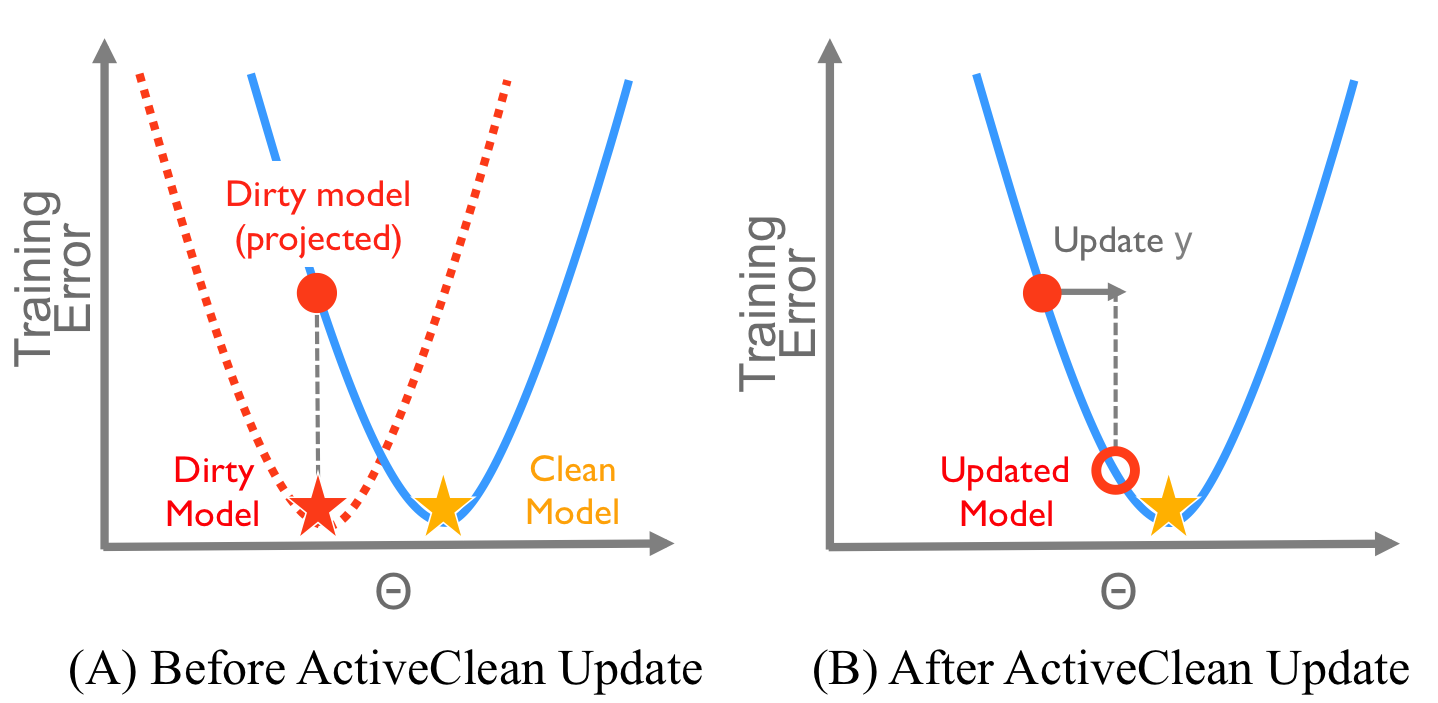
\includegraphics[width=\columnwidth]{figs/update-arch2.png}
 \caption{(A) A model trained on dirty data can be thought of as a sub-optimal point w.r.t to the clean data. (B) The gradient gives us the direction in which we need to move the suboptimal model to approach the true optimum. \label{update-arch2}}
\end{figure}

We want to get to the optimal clean model $\theta^{(c)}$ which is visualized as a yellow star.
The first question is which direction do we move $\theta$.
We do not know whether we need to move left or right.
For this class of models, given a suboptimal point, we can find the direction to 
the global optimum.
Mathematically, this direction corresponds to gradient of the loss function.
The gradient is a function of the clean data that returns a $d$-dimensional vector w.r.t the current dirty optimal model i.e., the direction between the dirty model and the true clean model.
We need to move some distance $\gamma$ along this direction (Figure \ref{update-arch2}b):
\[
\theta^{new} \leftarrow \theta^{(d)} - \gamma \cdot \nabla\phi(\theta^{(d)})
\]
In our visualization, this corresponds to whether we should move left or right.
At the optimal point, the expected gradient will be zero.
So intuitively, this approach iteratively moves the model downhill to, or corrects, the dirty model until the budget is reached.

However, in reality, we do not have the all of the clean data and have to approximate this gradient from a sample.
The intuition, which we will formalize in Section \ref{sgd}, is that if we are on average in the right direction the algorithm is guaranteed to converge with analytics bounds on the convergence rate.
It turns out that for an appropriately chosen $\gamma$, this convergence will hold for any batch size that we choose.

\subsection{Average Gradient From a Sample}
To derive a sample-based update rule, the first property that we should recognize is that sums commute with derivatives and gradients.
Our class of Machine Learning models are based on loss minimization, that is they are a sum of losses, so the gradient $\nabla\phi(\theta)$ is:
\[
\nabla\phi(\theta) = \frac{1}{n} \nabla\phi(x_i^{clean},y_i^{clean},\theta)
\]
We estimate this gradient from a sample by averaging over a sample of clean data and reweighting them by their sampling probability.
Let $S$ be a sample of data, where each $i \in S$ is drawn with probability $p_i$:
\[
\nabla\phi(\theta) \approx g_{S}(\theta) = \frac{1}{n\mid S \mid} \sum_{i \in S}\frac{1}{p_i}\nabla\phi(x_i^{clean},y_i^{clean},\theta)
\]
Then for every batch of data cleaned, we apply the update to the current best model estimate:
\[
\theta^{(t)} \leftarrow \theta^{(t-1)} - \gamma \cdot g_{S}(\theta^{(t-1)})
\]

The detection in the previous step adds a small complication, since the sample $S_{dirty}$ is not representative of all of the data.
We also have to compensate for this bias by averaging this estimate with the gradient with respect to the clean data:
\[
g_C(\theta) = \frac{1}{\mid R - R_{dirty}\mid}\sum_{i \in R - R_{dirty}}\nabla\phi(x_i^{clean},y_i^{clean},\theta)
\]
Then, for weights $\alpha,\beta$ which we will subsequently discuss how to select (Section \ref{params}):
\[
g(\theta) = \alpha \cdot g_C(\theta) + \beta \cdot g_S(\theta)
\]
This average represents a novel optimization for the data cleaning that is not studied in the stochastic optimization literature.
Since some data are less expensive to process than others, we can batch together processing the clean data and sample to process the dirty data.
Finally, we add in the iteration, and at each iteration $i$, the update becomes:
\[
\theta^{(i+1)} \leftarrow \theta^{(i)} - \gamma \cdot g(\theta^{(i)}) \blacksquare
\]

\subsection{Model Update Algorithm}
We propose the iterative model correction algorithm.
We initialize the algorithm with $\theta^{(d)}$ which is the dirty model.
At each iteration $i=\{1,...,t\}$, we clean a batch of data $b$ selected from the set of candidate dirty records $R_{dirty}$.
Then, starting with $\theta^{(d)}$, we apply an averaged gradient update to get $\theta^{(i)}$.
We iterate until our budget of cleaning $k = t \cdot b$ record is reached.

We present the model update algorithm here:
\begin{enumerate}[noitemsep]
	\item Calculate the gradient over the sample of clean data and call the result $g_S(\theta^{(i-1)})$
	\item Calculate the average gradient over all the data in $R_{clean}=R-R_{dirty}$, and call the result $g_C(\theta^{(i)})$
	\item Apply the following update rule:
	\[
	\theta^{(i+1)} \leftarrow \theta^{(i)} - \lambda \cdot(\alpha\cdot g_S(\theta^{(i)}) + \beta \cdot  g_C(\theta^{(i)}))
	\]
\end{enumerate} 

\subsubsection{Selecting the Parameters}\label{params}
We have to set the parameters $b$, $\lambda$, $\alpha$, $\beta$.
We will show that theory from the stochastic optimization literature can inform how to set these parameters.
First, we will review all of the parameters that need to be set.

\noindent\textbf{Batch Size $b$ : } The batch size $b$ controls the frequency of iteration. Larger batches provide a more accurate estimate of the gradient at each iteration but analyst gets less frequent model updates. 

\vspace{0.5em}

\noindent\textbf{Step Size $\gamma$ : } We have not explained how to pick the step size $\gamma$. In other words, how far should we travel in the gradient direction.

\vspace{0.5em}

\noindent\textbf{Weights $\alpha,\beta$ : } The next problem is deriving the proportions with which we should combine $g_S(\theta)$ and $g_C(\theta)$. It turns out that $\alpha = \frac{R_{clean}}{R}$ and $\beta = \frac{R_{dirty}}{R}$, and we will show a derivation below.

\vspace{0.5em}

\noindent\textbf{Choosing $S$: } As we mentioned, the optimal clean model depends on \emph{all} the clean data, not just a sample. 
So $g_S$ is an approximation of the true gradient $g^*$ with some error $g^* \pm \epsilon$. 
The quality of the update depends on how well we can approximate $g^*$ using $g_S$.
The problem is how should we construct the sample of data to clean $S$ to get the most accurate update.
In particular, how should we choose the sampling probabilities $p_i$ for each $i \in S$ such that the error is minimized.

\subsection{Analysis with Stochastic Gradient Descent}\label{sgd}
This update policy can be formalized as a class of very well studied algorithms called Stochastic Gradient Descent.
This gives us a theoretical framework to understand and analyze our update rule, bound the error, and choose points to clean.
Mini-batch stochastic gradient descent (SGD) is an algorithm for finding the optimal value
of $\theta$, given the convex loss, and data.
In mini-batch SGD, random subsets of data are selected at each iteration and the average gradient is computed for every batch.
The key difference is that in traditional SGD there is no notion of dirty and clean data, and we have to formalize our method as a variant of mini-batch SGD to apply the theory.

\vspace{0.5em}

\noindent\textbf{ \sys as Lazy SGD: } The update technique is \sys can be formalized as a variant of SGD that lazily materializes the clean value.
We apply SGD to dirty dataset, as data is sampled at each iteration, data is cleaned.
To the SGD algorithm it is as if the entire data is clean but we are lazily materializing the clean values.
It is well known that even for arbitrary initializations SGD makes significant progress in less than one epoch (a pass through the entire dataset) \cite{bottou2012stochastic}.
Furthermore in our setting, the dirty model can be much more accurate than an arbitrary initialization.
This is the property that we exploit to make significant progress by cleaning only a sample of data.

\vspace{0.5em}

\noindent\textbf{Deriving $\alpha$ and $\beta$: } We first want to show how to select $\alpha$ and $\beta$ such that our estimate of the gradient is unbiased. 
We will then show that SGD will converge when the estimate is unbiased and the step-size is chosen appropriately.
We first select a set of records before starting we select a set of dirty records $R_{dirty} \subseteq R$. 
We construct batch $S_{dirty}$ only from the dirty records and apply cleaning to this batch.
Now the problem is that this sample (and the resulting gradient) is possibly biased since we are excluding some data.
However, since we know that the set $R_{clean} = R - R_{dirty}$ is clean, we can compute the average gradient over those records without cleaning:
\[
g_C(\theta^{t}) = \frac{1}{\mid R - R_{dirty} \mid} \sum g_i(\theta^{t})
\]
Since we know the partition sizes, we can combine the two estimates $g_C$ and $g_S$ togther:
\[
g(\theta^{t}) = \frac{\mid R_{dirty} \mid \cdot g_S + \mid R_{clean} \mid \cdot g_C  }{\mid R \mid}
\]
Therefore,
\[
\alpha = \frac{R_{clean}}{R}, \beta = \frac{R_{dirty}}{R}
\]

\begin{lemma}
The gradient estimate $g(\theta^{t})$ is unbiased if $g_S$ is an unbiased estimate of:
\[
\frac{1}{\mid R_{dirty} \mid} \sum g_i(\theta^{t})
\]
\end{lemma}
\begin{proof}[Sketch]
This result follows directly from the linearity of expectation, since we are adding a deterministic result with an unbiased result.
\end{proof}

\vspace{0.5em}

\noindent\textbf{ Setting $\gamma$: } There is extensive literature in machine learning for choosing the step size $\gamma$ appropriately. $\gamma$ can be set either to be a constant or decayed over time. Many machine learning frameworks (e.g., MLLib, Sci-kit Learn, Vowpal Wabbit) automatically set learning rates or provide different learning scheduling frameworks. 
In our experiments, we use a technique called inverse scaling where there is a parameter $\gamma_0=0.1$, and at each iteration we reduce it to $\gamma_t = \frac{\gamma_0}{\mid S \mid t}$. 

\vspace{0.5em}

\noindent\textbf{ Convergence: } Convergence properties of batch SGD formulations has been well studied \cite{dekel2012optimal}. From the preceding analysis, we know that our gradient estimate is unbiased and we know how to select the step size.  

\begin{proposition}
For an appropriately chosen learning rate $\gamma_t$, batch stochastic gradient descent will converge if $\mathbb{E}(g_S)=g^*$.
\label{unbiased}
\end{proposition}

\vspace{0.5em}

\noindent\textbf{ Convergence Rate: } The convergence rates of SGD are also well analyzed \cite{dekel2012optimal,bertsekas2011incremental,zhao2014stochastic}. 
Suppose, a user cleans a batch size of $b$ examples at each iteration.
This allows us to bound the error of intermediate models and understand the expected number of steps before a model within a certain error. 

\begin{proposition}
For a general convex loss, a batch size $b$, and $t$ iterations, the convergence rate is bounded by $O(\frac{\sigma^2}{\sqrt{bt}})$. 
$\sigma^2$ is the variance in the estimate of the gradient at each iteration:
\[
\mathbb{E}(\|g_S - g^*\|^2)
\]
\end{proposition}

\vspace{0.5em}

\noindent\textbf{ Setting the batch size: } The batch size should be set by the analyst to have the desired properties.
Larger batches will take longer to clean and will make more progress towards the clean model, but will have less fequent model updates.
On the other hand, smaller batches are cleaned faster and have more frequent model updates but make less progress.
The overheads introduced by our approach are more evident at smaller batch sizes.
There are diminishing returns to increasing the batch size $O(\frac{1}{\sqrt{b}})$.
Empirically, we find that batch sizes of 50 converge the fastest on our data and we specify this parameter in our experiments.
If a data cleaning technique requires a larger batch size than this, i.e., data cleaning is fast enough that the iteration overhead is significant compared to cleaning 50 records, we can always apply the updates in smaller batches.
For example, the batch size set by the analyst might be $b=1000$, but we apply the model updates after every $50$ records are cleaned.
This way we can dissociate the requirements of SGD and the data cleaning technique.

\vspace{0.5em}

\noindent\textbf{ Non-covex losses: } We acknowledge that there is an increasing popularity of non-convex losses in the Neural Network and Deep Learning literature. 
However, even for these losses, gradient descent techniques still apply. 
Instead of converging to a global optimum they converge to a locally optimal value. 
Likewise, \sys will converge to the closest locally optimal value to the dirty model. 
Because of this, it is harder to reason about the results.
Different initializations will lead to different local optima, and thus, introduces a complex dependence on the initialization with the dirty model.
This problem is not fundemental to \sys and any gradient technique suffers this challenge for general non-convex losses, and we hope to explore this more in the future.


